\todo{parler également de l'accélération}

Pour pouvoir proposer de nouvelles fonctionnalités de prévention, il faut optimiser le tableau de bord. Il faut créer des logos communs à tous pour avoir le même langage. 

\todo{ajout d'un tableau de bord connecté avec des capteurs et des alertes en temps réel.}
L'idée serait d'intégrer dans les motos une puce GPS qui serait capable d'avertir en cas de virage dangeureux. L'alerte (sonore via un intercom et voyant au tableau de bord) serait envoyée via le tableau de bord connecté si la vitesse est supérieure à 5 km/h à la vitesse limite autorisée. Généralement, les virages sont signalés par des panneaux et par une limitation de vitesse. Des chercheurs Alex Liniger et Simon Hecker ont développé un prototype , Aegis Rider AG\cite{vitesse_virage_mcnews} permettant de prendre la meilleure trajectoire. Cependant, ce dernier ne prend pas en compte les autres facteurs de la route (autres usagers, état de la chaussée, etc.). 

\begin{figure}[h]
    \centering
    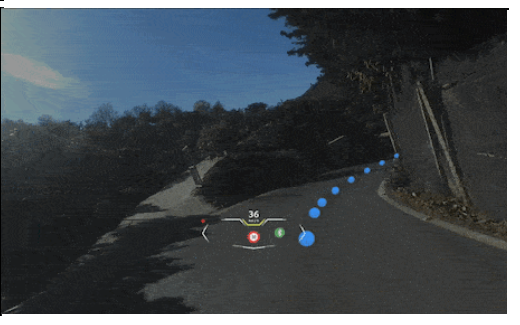
\includegraphics[width=0.7\textwidth]{coeur_memoire/images/aegis.png} 
    \caption{Prototype Aegis Rider AG pour la détection de virages dangereux.}
\end{figure}
Cette fonctionnalité est très interessante mais elle empêche une bonne visibilité de la surface de la route et elle peut fausser une prise de décision.
Comme illustré dans la Figure~\ref{fig:trajectoire_securite_difficulte}, le processus ne pourra pas adapter sur des virages dit "imparfaits".









\todo{voir pour faire une petite ligne de code ?}

\underline{Contexte:} En balade dans le 77, un motard roule sur une départementale. Dans cette situation, il est équipé d'un boitié GPS qui récupère ses coordonnées en temps réel. Il arrive dans une portion de virages limitée à 70 km/h nommée "Les 17 virages", près d'Arbonne-La-Forêt. Cette série de virages est dangeureuse car la route n'est pas bonne, n'est pas large et l'adhérence n'est pas optimale. De plus, il y a un virage dangereux à l'équerre qui surgit au milieu de cette série. La trajectoire de sécurité est fortement recommandé. Par expérience, avoisiner les 70 km/h est déjà bien au vue de la portion qui y est technique. 

\begin{figure}[H]
    \centering
    \includegraphics[width=0.7\textwidth]{coeur_memoire/schéma/Capture d’écran 2025-07-24 à 15.45.48.png} 
    \caption{Point GPS des 17 virages.}
\end{figure}

\todo{photo des 17 virages}



Les coordnnées GPS sont : 48.385171, 2.563108.

\todo{mettre le diagramme}
Voici le diagramme d'action de cette fonctionnalité:\\

\begin{figure}[H]
    \centering
    \includegraphics[width=0.8\textwidth]{coeur_memoire/schéma/Capture d’écran 2025-07-24 à 17.48.10.png} 
    \caption{Diagramme d'action du Système de prévention de virages dangereux}
\end{figure}

Pour réaliser un bout de code sur cette fonctionnalité, j'ai décidé d'utiliser ces bibliothèques :\\
• osmnx\cite{osm_doc} : permet d’interroger OSM (OpenStreetMap) et de récupérer des graphes routiers.\\
•	geodesic (de geopy \cite{geopy}) : mesure la distance réelle (en mètres) entre 2 points GPS.\\

L'interêt de calculer la courbure de la courbe est de pouvoir anticiper le virage et par conséquent, adapter la vitesse pour optimiser l'adhérence, la trajectoire où l'on se sentira le plus en sécurité. \\
Le calcul de la courbure permettra d'identifier un virage s'il est dangereux à partir de données GPS cartographiques pour enfin adapter le comportement du système embarqué (alerte, adaptation de trajectoire, assistance..).
Donc la courbure mesure à quel point une route peut changer de direction sur une courte distance, ici, dans un virage.\\
Une route droite a une courbure environ égale à 0. Une route qui tourne fort (virage serré) a une courbure élevée.

\begin{table}[ht]
\centering
\begin{tabular}{|l|c|c|c|}
\hline
Route & Rayon du virage & Courbure (simplifiée) & Risque \\
\hline
ligne droite & infini & 0 & faible \\
Virage large autoroute & 500 m & Faible (0.01) & faible \\
Virage serré en montagne & 30 m & Forte (0.1–0.2) & Élevé \\
\hline
\end{tabular}
\caption{Exemple en pratique}
\end{table}

Un virage serré avec une courbure > 0.1 est souvent dangereux à +60 km/h, surtout à moto.
Plusieurs études indiquent que les rayons < 50 m sont classés comme virages dangereux pour les motos. À plus de 60 km/h, une moto doit pencher à plus de 35°à 40° dans le virage ce qui augmente énormément le risque de chute, surtout s’il y a du gravier, pluie, vent latéral…
L’estimation “courbure > 0.1 = danger > 60 km/h” est une règle empirique, basée sur des données de sécurité moto reonnues, des normes d'ingénierie routière et des approximations géométriques issues de GPS.


L'avantage d'avoir un calcul automatique et en amont, cela permet de prévenir avant même d'être dans le virage. Il peut remplacer un panneau quand celui-ci n'est pas visible. Elle ne remplace pas une analyse dynamique complète mais elle est suffisante pour alerter automatiquement le pilote ce qui est exactement l’objectif du système.



\begin{tcolorbox}[title=Calcul de la courbure]
Courbure mathématique\cite{formule_curvature} d’un virage:
\[
courbure\_virage = \kappa = \frac{1}{R}
\]
où R est le rayon du virage\\
Forme simplifiée de la courbure basée sur la déviation par rapport à une ligne droite.\\
a, b et c sont trois points dans la courbe.\\
\[
curvature = abs((a + b - c) / (a + b))
\]
a + b = distance réelle parcourue en suivant la route \\
c = distance directe entre le début et la fin (comme si on traçait une corde)
\end{tcolorbox}

\begin{figure}[H]
    \centering
    \includegraphics[width=0.7\textwidth]{coeur_memoire/schéma/Capture d’écran 2025-07-22 à 16.27.35.png} 
    \caption{Schéma présentant une moto avant un virage}
\end{figure}


\todo{illustration, développement}

\todo{Détailler le code}

\lstinputlisting[language=Python]{coeur_memoire/programme1.py}

L'idée maintenant est de prévenir l'usager d'un logo universel. Évidemment, la disposition sera optimisée pour chaque écran. 
\begin{figure}[H]
    \centering
    \includegraphics[width=0.6\textwidth]{coeur_memoire/images/Capture d’écran 2025-07-25 à 14.42.42.png} 
    \caption{Génération d'un tableau de bord possible avec l'IA.}
\end{figure}

